%%
%% File:    thesis.tex
%%
%% Use:     Template file for a UNR Thesis/Dissertation
%%
%% Creator: Alex Fiannaca
%%          Human-Computer Interaction Lab
%%          Department of Computer Science & Engineering
%%          University of Nevada - Reno
%%          fiannac4@live.com
%%          www.alifeincode.com
%%
%% Note:    This sample thesis file was originally created by Blake Jacquot and Andrew Myers
%%          from Cornell. It has been significantly altered to meet the formatting guidelines
%%          of the UNR Grad School. That being said, this template is NOT AN OFFICIAL template
%%          from the UNR Grad School. Please be sure to double check all formatting requirements 
%%          for yourself before attempting to submit your work! This document/class is provided
%%          with no warranty or guarantee of correctness! It is simply intended as a helpful 
%%          starting place for UNR grad students.
%%

% Options: [master] (thesis formatting) / [phd] (dissertation formatting)
%          [tocprelim] (adds roman numeral pages to the table of contents)
\documentclass[master,tocprelim]{unrthesis}

%
% tocprelim option must be included to put the roman numeral pages in the
% table of contents
%
% This sample document was originally provided by Blake Jacquot and Andrew 
% Myers (Cornell). It has since been updated to provide for the requirements
% of the UNR grad school.
%

% Some possible packages to include
\usepackage{graphicx,pstricks}
\usepackage{graphics}
\usepackage{moreverb}
\usepackage{subfigure}
\usepackage{epsfig}
\usepackage{subfigure}
\usepackage{txfonts}
\usepackage{lipsum}
\usepackage{tikz}
\usepackage{pgfplots}
\usepackage{algorithm}
\usepackage{algpseudocode}

% Set an appropriate font. Palatino is much nicer than Times...
\usepackage{palatino}

% The hangcaption package will create more sensible caption wrapping (single spaced, 2nd line indents)
\usepackage{hangcaption}
\renewcommand{\caption}[1]{\singlespacing\hangcaption{#1}\normalspacing}

% If you're having problems with overfull boxes, you may need to increase the tolerance to 9999
% \tolerance=9999

% REQUIRED: Set the general thesis fields for generating the title page and committee page
\title{Your Title Goes Here}
\author{John Doe}
\advisor{Dr. Jack Smith}
\conferraldate{May}{2014}                          % Month can only be: May, August, or December
\masterstype{Science}                              % Science, Arts, Business Administration, etc...
\degreefield{Computer Science and Engineering}
\copyrightholder{John Doe}                         % Typically this is the same as the author
\copyrightyear{2014}

\begin{document}

% REQUIRED: Create the title page for the thesis/dissertation
\maketitle

% OPTIONAL: Create a copyright page
\makecopyright

% REQUIRED: Create the committee approval page (addgraduatedean must be the last call!)
\addcommitteemember{Jack Smith}{Ph.D.}{Advisor}                           % Add committee members, then the
\addcommitteemember{Jake Johnson}{Ph.D.}{Committee Member}                % dean last. Members will appear on
\addcommitteemember{Janny Jackson}{Ph.D.}{Graduate School Representative} % the committee page in the order
\addgraduatedean{Marsha H. Read}{Ph.D.}                                   % declared here
\makecommitteepage

% REQUIRED: Create the abstract page
\begin{abstract}
\lipsum[1]

\end{abstract}

% OPTIONAL: Create a dedication page
\begin{dedication}
This document is dedicated to those graduate students everywhere who are trudging through the black abyss that is thesis/dissertation writing. \newline
May peace be with you.

\end{dedication}

% OPTIONAL: Create an acknowledgements page
\begin{acknowledgements}
\lipsum[2]

Oh, and of course, I would like to thank the academy...

\end{acknowledgements}

% REQUIRED: Create the Table of Contents, List of Tables, and List of Figures
\contentspage
\tablelistpage
\figurelistpage

% REQUIRED: Create the actual manuscript of the thesis/dissertation
\begin{manuscript}

% Use chapters and sections in the usual manner for organizing your writing
\chapter{Introduction to Faster-Than-Light Travel}

\section{Relativity? Who Cares?}
This section, while highly provocative, is quite small, and leaves something to be desired. Importantly, you can see that sections run together and do not cause page breaks like chapters do.

\section{Algorithms for Attempting the Leap Outside}
There are many ways to divide your paper down into a logical structure. Lets take a look at this in depth.

\subsection{No, Really, It's Totally Possible}
"In depth" was intended quite literally actually. The depth increases as we move into subsections like this one. Surprisingly we aren't done yet, though.

\subsubsection{Some Fine Details}
Do people really need sub-sub-sections? Well if you do, then here is how it will look.

\section{Math and Figures Look Nice}
Did you know math could look so fun? The dielectric constant at the air-metal interface
determines the resonance shift as absorption or capture occurs.

\begin{equation}
k_1=\frac{\omega }{c({1/\varepsilon_m + 1/\varepsilon_i})^{1/2}}=k_2=\frac{\omega
sin(\theta)\varepsilon_{air}^{1/2}}{c}
\end{equation}

\noindent
where $\omega$ is the frequency of the plasmon, $c$ is the speed of
light, $\varepsilon_m$ is the dielectric constant of the metal,
$\varepsilon_i$ is the dielectric constant of neighboring insulator,
and $\varepsilon_{air}$ is the dielectric constant of air.

% Example table to be displayed in the table list
\begin{table}[h]
    \begin{center}
        \begin{tabular}{|c|c|c|}
            \hline
            Column One & Column Two & Column Three \\ \hline
            a          & b          & c            \\ \hline
            1          & 2          & 3            \\ \hline
            x          & y          & z            \\ \hline
        \end{tabular}
    \end{center}
    \label{table:table1}
    \caption{Some Interesting Data Set}
\end{table}

% Example figure to be displayed in the figure list. pgfplots works nicely for generating graphs
\begin{figure}[h]
    \begin{center}
        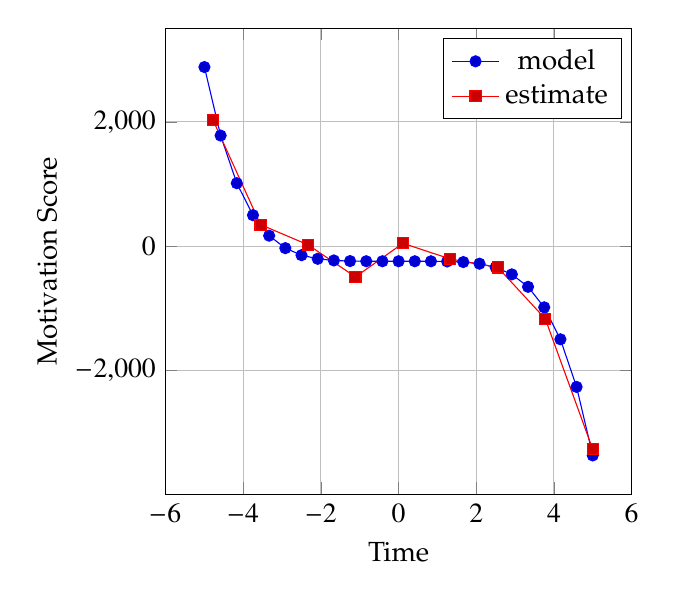
\begin{tikzpicture}
        	\begin{axis}[
        		height=7.5cm,
        		width=7.5cm,
        		grid=major,
        		ylabel=Motivation Score,
        		xlabel=Time
        	]
            	\addplot {-x^5 - 242};
            	\addlegendentry{model}
            
            	\addplot coordinates {
            		(-4.77778,2027.60977)
            		(-3.55556,347.84069)
            		(-2.33333,22.58953)
            		(-1.11111,-493.50066)
            		(0.11111,46.66082)
            		(1.33333,-205.56286)
            		(2.55556,-341.40638)
            		(3.77778,-1169.24780)
            		(5.00000,-3269.56775)
            	};
            	\addlegendentry{estimate}
        	\end{axis}
        \end{tikzpicture}
    \end{center}
    \label{figure:figure1}
    \caption{Thesis Writing Motivation Over Time}
\end{figure}

\chapter{Alice in Wonderland}

\section{The Black Kitten}
  One thing was certain, that the WHITE kitten had had nothing to
do with it:---it was the black kitten's fault entirely~\cite{aiw}.  For the
white kitten had been having its face washed by the old cat for
the last quarter of an hour (and bearing it pretty well,
considering); so you see that it COULDN'T have had any hand in
the mischief.

  The way Dinah washed her children's faces was this:  first she
held the poor thing down by its ear with one paw, and then with
the other paw she rubbed its face all over, the wrong way,
beginning at the nose:  and just now, as I said, she was hard at
work on the white kitten, which was lying quite still and trying
to purr---no doubt feeling that it was all meant for its good.

  But the black kitten had been finished with earlier in the
afternoon, and so, while Alice was sitting curled up in a corner
of the great arm-chair, half talking to herself and half asleep,
the kitten had been having a grand game of romps with the ball of
worsted Alice had been trying to wind up, and had been rolling it
up and down till it had all come undone again; and there it was,
spread over the hearth-rug, all knots and tangles, with the
kitten running after its own tail in the middle.

\section{The Reproach}

  `Oh, you wicked little thing!' cried Alice, catching up the
kitten, and giving it a little kiss to make it understand that it
was in disgrace.  `Really, Dinah ought to have taught you better
manners!  You OUGHT, Dinah, you know you ought!' she added,
looking reproachfully at the old cat, and speaking in as cross a
voice as she could manage---and then she scrambled back into the
arm-chair, taking the kitten and the worsted with her, and began
winding up the ball again.  But she didn't get on very fast, as
she was talking all the time, sometimes to the kitten, and
sometimes to herself.  Kitty sat very demurely on her knee,
pretending to watch the progress of the winding, and now and then
putting out one paw and gently touching the ball, as if it would
be glad to help, if it might.

  `Do you know what to-morrow is, Kitty?' Alice began.  `You'd
have guessed if you'd been up in the window with me---only Dinah
was making you tidy, so you couldn't.  I was watching the boys
getting in stick for the bonfire---and it wants plenty of
sticks, Kitty!  Only it got so cold, and it snowed so, they had
to leave off.  Never mind, Kitty, we'll go and see the bonfire
to-morrow.'  Here Alice wound two or three turns of the worsted
round the kitten's neck, just to see how it would look:  this led
to a scramble, in which the ball rolled down upon the floor, and
yards and yards of it got unwound again.

  `Do you know, I was so angry, Kitty,' Alice went on as soon as
they were comfortably settled again, `when I saw all the mischief
you had been doing, I was very nearly opening the window, and
putting you out into the snow!  And you'd have deserved it, you
little mischievous darling!  What have you got to say for
yourself?  Now don't interrupt me!' she went on, holding up one
finger.  `I'm going to tell you all your faults.  Number one:
you squeaked twice while Dinah was washing your face this
morning.  Now you can't deny it, Kitty:  I heard you!  What that
you say?' (pretending that the kitten was speaking.)  `Her paw
went into your eye?  Well, that's YOUR fault, for keeping your
eyes open---if you'd shut them tight up, it wouldn't have
happened.  Now don't make any more excuses, but listen!  Number
two:  you pulled Snowdrop away by the tail just as I had put down
the saucer of milk before her!  What, you were thirsty, were you?

\end{manuscript}

% OPTIONAL: Create a sample appendix with one chapter
\begin{appendices}
\chapter{Proof of the SSL (Stupid Silly Lemma)}
Don't you just love writing proofs? Maybe this proof requires an algorithm. Lets take a look at an algorithm. Clearly there are some formatting issues in the algorithm/algorithmic environment. I'm still working on fixing these issues...


\begin{algorithm}
    \label{euclid}
    \caption{Euclid’s algorithm}
    \begin{algorithmic}[1]
        \Procedure{Euclid}{$a,b$}\Comment{The g.c.d. of a and b}
            \State $r\gets a\bmod b$
            \While{$r\not=0$}\Comment{We have the answer if r is 0}
            \State $a\gets b$
            \State $b\gets r$
            \State $r\gets a\bmod b$
            \EndWhile\label{euclidendwhile}
            \State \textbf{return} $b$\Comment{The gcd is b}
            \EndProcedure
    \end{algorithmic}
\end{algorithm}

\end{appendices}

% REQUIRED: Create the bibliography using the BibTeX file thesis.bib
\bibliography{thesis}

\end{document}
